\chapter{Evaluation und Validation}
\label{ch:Eval}

Um das System zu validieren und die Grenzen der Infrarotbildverarbeitung in diesem Gebiet zu ermitteln wurden einige Experimente durchgeführt. Diese Experimente zeigen, was das System kann und wo die Grenzen des Systems und auch der Infrarottechnik liegen.\\
\\
\section{Erklärungen}
\label{sec:explanation}
In diesem Kapitel werden Test statistisch ausgewertet und analysiert. Dazu werden hier die wichtigsten Begriffe und Konzepte erklärt.

\subsection{Farbcodierung}
Zur Auswertung der Experimente werden Bilder mit Markierungen verwendet. Diese sind wie folgt Farbcodiert.\\

\begin{itemize}
	\item \textbf{Grün:} Korrekt gefundene Person (True Positive)
	\item \textbf{Gelb:} Nicht gefundene Person (False Negative)
	\item \textbf{Rot:} Nichtiger Treffer (False Positive)
\end{itemize}
\vspace{1em}

\subsection{Begriffserklärung}
\noindent In dem Kapitel werden die folgenden Fachbegriffe verwendet:
\begin{itemize}
	\item $True\: Positive:$   Person wurde korrekt Identifiziert
	\item $True\: Negative:$   Hintergrund oder fremde Wärmequelle wurde \textbf{nicht} als Person identifiziert. Diese werden in diesem Kapitel nicht weiter verwendet, da diese der standard Fall ist und nicht spezifisch ausgewertet werden kann.
	\item $False\: Positive:$  Hintergrund oder fremde Wärmequelle wurde als Person identifiziert
	\item $False\: Negative:$  Person wurde nicht erkannt.
\end{itemize}
\vspace{1em}

\subsection{Statistische Metriken}
\noindent Zudem werden die folgenden Metriken verwendet, diese sind leicht angepasst, da die Klasse True Negative fehlt:

\begin{itemize}
	\item \textbf{Precision:} Korrekte Treffer / Alle Treffer\[\dfrac{True\: Positive}{True\: Positive + False\: Positive}\]
	\item \textbf{Recall/Accuracy:} Korrekte Treffer / Anzahl Personen\[\dfrac{True\: Positive}{True\: Positive + False\: Negative}\]
	\item \textbf{F1-Score:} \[\dfrac{2*Precision*Recall}{Precision + Recall}\]
\end{itemize}


\section{Vergleich mit Anforderungen}
\label{sec:VergleichAnforderungen}

Der erforderte Stand der Technik wurde in Kapitel \ref{ch:StandDerTechnik} präsentiert. Die gefundenen Algorithmen wurden in Kapitel \ref{ch:ideasAndConcepts} erklärt und evaluiert.\\
Das erste Hauptziel war es ein lauffähiges System zu entwickeln, welches die Position und Anzahl der Personen in einem Infrarotbild bestimmen kann. Dieses Ziel wurde mit einem Recall von 91.5\%  erreicht (siehe Tabelle \ref{tbl:stat}). Die beim betrachten der Werte in Tabelle \ref{tbl:results} und \ref{tbl:stat} ist zu beachten, dass dabei auch die Grenzen des Systems getestet wurden. So zum Beispiel in Kapitel \ref{sec:cloths} wo der Einfluss isolierender Kleidung analysiert wird.\\
Das zweite Hauptziel ist es Schwierigkeiten bei der Lösung der Aufgabe zu erläutern und Lösungsmöglichkeiten dazu vorzuschlagen. Dies wird in diesem Kapitel und im Kapitel \ref{ch:Ausblick} erfüllt.

% Tabelle mit ergebnissen
{
	\renewcommand{\arraystretch}{1.3}
	
	\begin{table}[H]
		\scriptsize
		\centering
		\begin{tabularx}{.5\textwidth}{Xrr}\\
			\hline
			\multicolumn{3}{c}{\textbf{Ergebnisse der Algorithmen}}\\
			\hline
			\textbf{Kategorien} & \textbf{CNN} & \textbf{Threshold}\\
			\hline
			\textit{Anzahl verwendeter Aufnahmen} & 323 & 323\\
			\hline 
			\textit{Gesamtanzahl Personen in Bilder} & 718 & 718\\
			\hline
			\textit{True Positive} & 657 & 650\\
			\hline
			\textit{False Positive} & 120 & 142\\
			\hline
			\textit{False Negative} & 61 & 68\\
		\end{tabularx}
		\caption{Zusammenfassung der Ergebnisse beider Algorithmen}
		\label{tbl:results}
	\end{table}
	\begin{table}[H]
		\scriptsize
		\centering
		\begin{tabularx}{.5\textwidth}{Xrr}
			\hline
			\multicolumn{3}{c}{\textbf{Statistische Auswertung}}\\
			\hline
			\textbf{Kategorien} & \textbf{CNN} & \textbf{Threshold}\\
			\hline
			\textit{Recall} & 91.5\% & 90.5\%\\
			\hline  
			\textit{Precision} & 84.5\% & 82.1\%\\
			\hline
			\textit{F1-Score} & 87.9\% & 86.1\%\\
			\hline
		\end{tabularx}
		\caption{Statistische Auswertung der Performance beider Algorithmen}
		\label{tbl:stat}
	\end{table}
}

\section{Fremde Wärmequellen}
\label{sec:FremdeWärmequellen}

In diesem Versuch wurde der Einfluss von fremden Wärmequellen, wie zum Beispiel Laptops, Natels, Kaffees oder Radiatoren, evaluiert. Dabei wurde der Effekt von Störquellen mit und ohne Personen im Raum analysiert.

\subsection{Versuchsaufbau}

Um die Performance der Algorithmen spezifisch in Bezug auf fremde Wärmequellen zu testen, wurden verschiedene Testsituationen erzeugt. Zuerst wurden fünf Laptops, von 13" bis 17",auf den Sitzungstisch gestellt, um zu sehen, ob Laptops ohne Personen Treffer generieren. Die Geräte wurden auf den gesamten Kamerawinkel verteilt, vom Zentrum des Bildes bis an den Rand. Da die Algorithmen nicht durch die Anzahl Wärmequellen, sondern nur durch die Distanz zwischen den Wärmequellen beeinflusst werden, konnte der ganze Kamerawinkel in einem einzigen Versuch getestet werden.\\
Die Temperatur der Laptops wurde von der Infrarotkamera als ca. 25\degree C erfasst, somit etwas unter der Abstrahlungswärme einer Person. Die Hauttemperatur einer Person wird von den Infrarotkameras zwischen 27\degree C und 33\degree C gemessen, je nach Kleidung und Behaarung.\\
Danach nahmen fünf Personen bei den Laptops platz,  ohne dass die Laptops verschoben wurde. Um zu testen, ob False Positives generiert werden, wenn jemand den Laptop bedient, die Arme zum Laptop reichen.\\
Um auch Wärmere Laptops überprüfen zu können wurde Bilder während einer Besprechung aufgezeichnet. Dabei war ein Laptop, dessen Temperatur im Bereich der Hauttemperatur einer Person liegt, in der Mitte des Tischs, ein anderer nahe bei einer Person. Die Szene ist in Abbildung \ref{fig:exampleDeviceTest2} zu sehen.
\\
\begin{figure}[htb]
	\centering
	\begin{subfigure}{.45\linewidth}
		\centering
		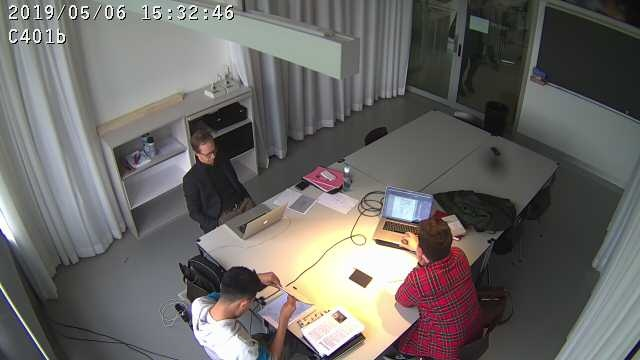
\includegraphics[keepaspectratio, height=4cm]{groundDeviceTest2}
	\end{subfigure}
	\begin{subfigure}{.45\linewidth}
		\centering
		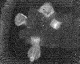
\includegraphics[keepaspectratio, height=4cm]{exampleDeviceTest2}
	\end{subfigure}
	\caption{Ansicht des Sitzungszimmers während der Aufnahme des zusätzlichen Laptop- und Personen-Testsets}
	\label{fig:exampleDeviceTest2}
\end{figure}
Schon bei der Erstellung der Modelle wurde ersichtlich, dass das Herausfiltern von Wärmequellen mit sehr kleiner Fläche für beide Algorithmen kein Problem darstellt. Aus diesem Grund wurden die Versuche mit kleineren Wärmequellen nur in kleinem Rahmen durchgeführt. Es wurde Test mit einem Mobiltelefon durchgeführt, in dem ein Natel an verschiedenen Postionen auf den Tisch gelegt wurde. Da Mobiltelefone meist in der Hosentasche getragen werden, weisen diese Temperaturen bis zu 34\degree C auf.\\
\\

\subsection{Resultate}

{
	\renewcommand{\arraystretch}{1.3}
	\begin{table}[H]
		\centering
		\scriptsize
		\begin{tabularx}{.9\textwidth}{Xrrrr}
			\hline
			\multicolumn{5}{c}{\textbf{\gls{CNN} Ergebnisse Fremde Wärmequellen}}\\
			\hline
			\textbf{Metriken} & \textbf{Nur Laptops} & \textbf{Laptops mit Personen} & \textbf{Mobiltelefon} & \textbf{Radiator}\\
			\hline 
			\textbf{Gesamtanzahl Personen in Bilder} & 0 & 39 & 0 & 20\\
			\hline
			\textbf{Korrekt identifizierter Personen} & 0 & 39 & 0 & 20\\
			\hline
			\textbf{Falsche Treffer} & 1 & 0 & 0 & 27\\
			\hline
			\textbf{Nicht erkannte Personen} & 0 & 0 & 0 & 0\\
			\hline
			\textbf{Recall} & -- & 100\% & -- & 100\%\\
			\hline  
			\textbf{Precision} & -- & 100\% & -- & 42.6\%\\
			\hline
			\textbf{F1-Score} & -- & 100\% & -- & 59.7\%\\
			\hline
		\end{tabularx}
		\caption{Ergebnisse des \gls{CNN}, der Experimente mit fremden Wärmequellen}
		\label{tbl:heatSourcesCNN}
	\end{table}
	\begin{table}[H]
		\centering
		\scriptsize
		\begin{tabularx}{.9\textwidth}{Xrrrr}
			\hline
			\multicolumn{5}{c}{\textbf{Threshold-Methode Ergebnisse Fremde Wärmequellen}}\\
			\hline
			\textbf{Metriken} & \textbf{Nur Laptops} & \textbf{Laptops mit Personen} & \textbf{Mobiltelefon} & \textbf{Radiator}\\
			\hline 
			\textbf{Gesamtanzahl Personen in Bilder} & 0 & 39 & 0 & 20\\
			\hline
			\textbf{Korrekt identifizierter Personen} & 0 & 33 & 0 & 20\\
			\hline
			\textbf{Falsche Treffer} & 1 & 014 & 16 & 87\\
			\hline
			\textbf{Nicht erkannte Personen} & 0 & 0 & 0 & 0\\
			\hline
			\textbf{Recall} & -- & 84.6\% & -- & 100\%\\
			\hline  
			\textbf{Precision} & -- & 70.2\% & -- & 18.7\%\\
			\hline
			\textbf{F1-Score} & -- & 76.7\% & -- & 31.5\%\\
			\hline
		\end{tabularx}
		\caption{Ergebnisse, der Threshold-Methode, der Experimente mit fremden Wärmequellen}
		\label{tbl:heatSourcesThresh}
	\end{table}
}

\subsection{Evaluation}

Die Threshold-Methode kann, wie erwartet, nicht gut mit anderen Wärmequellen umgehen. Dies, weil die Threshold-Methode nur durch Temperatur und Mindestgrösse eines Objekts entscheiden kann, ob es sich um eine Person handelt oder nicht. Deshalb hatte dieser auf den Testbildern mit Personen und Laptops, nur eine Precision Score von 70\% erreicht und bei dem Versuch mit Radiator auf hoher Stufe sogar nur eine von 18.7\% (Siehe Abbildungen  \ref{fig:ThreshPersonLaptop} und \ref{fig:thresholdRadiator}).\\
\\
Das \gls{CNN} kann gut mit anderen Wärmequellen umgehen, solange diese in ähnlicher Form antrainiert wurden (siehe Abbildung \ref{fig:cnnPersonLaptop}. Ist dies jedoch nicht der Fall und die Wärmequelle ist dem \gls{CNN} nicht in ähnlicher Form bekannt tendiert es dazu diese, wenn sie etwas grösser sind, als Personen zu identifizieren, was in Abbildung \ref{fig:cnnRadiator} zu sehen ist. Eine Lösung zu diesem Problem wird in Kapitel \ref{ch:Ausblick} diskutiert. 

\vspace{.5em}
\begin{figure}[htb]
	\centering
	\begin{subfigure}{.45\linewidth}
		\centering
		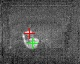
\includegraphics[keepaspectratio,height=4cm]{ThreshPersonLaptop}
		\caption{Ergebnis der Threshold-Methode des Experiments mit Laptop und Person}
		\label{fig:ThreshPersonLaptop}
	\end{subfigure}\hfill%
	\begin{subfigure}{.45\linewidth}
		\centering
		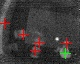
\includegraphics[keepaspectratio,height=4cm]{threshRadiator}
		\caption{Threshold-Methode Ergebnis des Radiator Experiments}
		\label{fig:thresholdRadiator}
	\end{subfigure}\hfill%
	\begin{subfigure}{.45\linewidth}
		\centering
		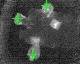
\includegraphics[keepaspectratio,height=4cm]{cnnPersonLaptop}
		\caption{CNN Ergebnis des Experiments mit Laptops und Personen}
		\label{fig:cnnPersonLaptop}
	\end{subfigure}\hfill%
	\begin{subfigure}{.45\linewidth}
		\centering
		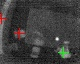
\includegraphics[keepaspectratio, height=4cm]{cnnRadiator}
		\caption{CNN Ergebnis des Radiator Experiments}
		\label{fig:cnnRadiator}
	\end{subfigure}\hfill%
	\begin{subfigure}{.55\linewidth}
		\centering
		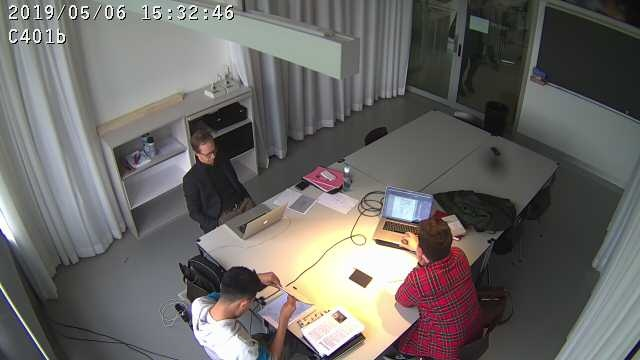
\includegraphics[keepaspectratio,height=3cm]{groundDeviceTest2}
		\caption{Ground-Truth des Experiments mit Laptop und Person}
		\label{fig:groundPersonLaptop}
	\end{subfigure}
	\caption{Experimente mit fremden Wärmequellen}
	\label{fig:HeatSources}
\end{figure}
\vspace{.5em}



\section{Distanz}
\label{sec:distanz}

Die Distanz zwischen zwei Personen ist ein wichtiger Faktor, der auf beide Algorithmen Einfluss hat. Da bei dem \gls{CNN} mit einer Sliding-Window Methode und Clustern der Treffer gearbeitet wird, kann das System, bei Personen, welche zu wenig Abstand zueinander haben, die Treffer nicht mehr auseinanderhalten. Bei der Threshold-Methode wird die Silhouette der Personen leicht vergrössert, wodurch mehrere Personen bei geringem Abstand als einzelner Treffer gewertet werden können.

\subsection{Versuchsaufbau}

Es wurden vier Personen in zwei Paaren so platziert, dass sich das eine Paar in einem idealen Winkel zur Infrarotkamera aufhält und das andere Paar in einem möglichst schwierigen Winkel. Dies ist in Abbildung \ref{fig:cnnDistance10} gut zu sehen. Zwei Personen sind deutlich voneinander getrennt, die anderen zwei überlappen sich aufgrund des Kamerawinkels. Diese Versuchsanordnung wurde gewählt, um in einem Test beide Extreme überprüfen zu können. 
Beim Test wurde schrittweise der Abstand zwischen den Testpersonen erhöht, um festzustellen, ab welcher Distanz die Algorithmen erfolgreich die Personen erkennen. Der Abstand wird in 10cm Schritten erhöht, weil 10cm auf Tischhöhe ca. einem Pixel auf dem Bild entspricht.

\subsection{Resultate}

{
	\renewcommand{\arraystretch}{1.3}
	\begin{table}[H]
		\centering
		\scriptsize
		\begin{tabularx}{.9\textwidth}{Xrrrrrr}
			\hline
			\multicolumn{7}{c}{\textbf{\gls{CNN} Ergebnisse Distanz Experiment}}\\
			\hline
			\textbf{Metriken} & \textbf{10cm} & \textbf{20cm} & \textbf{30cm} & \textbf{40cm} & \textbf{50cm} & \textbf{60cm}\\
			\hline 
			\textbf{Gesamtanzahl Personen in Bilder} & 29 & 18 & 54 & 18 & 51 & 28\\
			\hline
			\textbf{Korrekt identifizierter Personen} & 29 & 18 & 54 & 18 & 51 & 28\\
			\hline
			\textbf{Falsche Treffer} & 0 & 0 & 0 & 0 & 0 & 0\\
			\hline
			\textbf{Nicht erkannte Personen} & 0 & 0 & 0 & 0 & 0 & 0\\
			\hline
			\textbf{Recall} & 100\% & 100\% & 100\% & 100\% & 100\% & 100\%\\
			\hline  
			\textbf{Precision} & 100\% & 100\% & 100\% & 100\% & 100\% & 100\%\\
			\hline
			\textbf{F1-Score} & 100\% & 100\% & 100\% & 100\% & 100\% & 100\%\\
			\hline
		\end{tabularx}
		\caption{Ergebnisse des \gls{CNN}, der Distanz Experimente}
		\label{tbl:distanceCNN}
	\end{table}
	\begin{table}[H]
		\centering
		\scriptsize
		\begin{tabularx}{.9\textwidth}{Xrrrrrr}
			\hline
			\multicolumn{7}{c}{\textbf{Threshold-Methode Ergebnisse Distanz Experiment}}\\
			\hline
			\textbf{Metriken} & \textbf{10cm} & \textbf{20cm} & \textbf{30cm} & \textbf{40cm} & \textbf{50cm} & \textbf{60cm}\\
			\hline 
			\textbf{Gesamtanzahl Personen in Bilder} & 29 & 18 & 54 & 18 & 51 & 28\\
			\hline
			\textbf{Korrekt identifizierter Personen} & 22 & 15 & 54 & 18 & 51 & 28\\
			\hline
			\textbf{Falsche Treffer} & 4 & 1 & 3 & 1 & 3 & 1\\
			\hline
			\textbf{Nicht erkannte Personen} & 7 & 3 & 0 & 0 & 0 & 0\\
			\hline
			\textbf{Recall} & 75.9\% & 83.3\% & 100\% & 100\% & 100\% & 100\%\\
			\hline  
			\textbf{Precision} & 84.6\% & 93.8\% & 94.7\% & 94.7\% & 94.4\% & 100\%\\
			\hline
			\textbf{F1-Score} & 80.0\% & 88.2\% & 97.2\% & 97.2\% & 97.1\% & 100\%\\
			\hline
		\end{tabularx}
		\caption{Ergebnisse, der Threshold-Methode, der Distanz Experimente}
		\label{tbl:distanceThresh}
	\end{table}
}

\subsection{Evaluation}


Das \gls{CNN} Kann bereits ab einem Abstand von 10cm zuverlässig Personen auseinanderhalten.\\
Die Threshold-Methode kann Personen bereits ab einem Abstand von 10cm auseinanderhalten, sofern die Personen so ausgerichtet sind, dass die optische Verzerrung keinen Einfluss auf den Zwischenraum hat. Wie in der Abbildung \ref{fig:thresholdDistance10} in der linken Bildhälfte zu sehen ist, können die Personen, die auf die Kamera ausgerichtet sind, unterschieden werden. Sind die Person jedoch so platziert, wie auf der rechten Bildhälfte zu sehen ist, sind diese von der Kamera aus gesehen, hintereinander. Bei dieser geringen Distanz kann der Algorithmus deshalb nicht mehr bestimmen, ob es sich um eine oder mehrere Personen handelt.\\
Befinden sich die Personen in der schlechtestmöglichen Position, benötigt die Threshold-Methode einen Mindestabstand von 30cm, um die Personen fehlerfrei unterscheiden zu können (siehe Abbildung \ref{fig:thresholdDistance30}).

\begin{figure}[H]
	\begin{subfigure}{.45\linewidth}
		\centering
		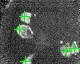
\includegraphics[keepaspectratio,height=4cm]{CNNDistance10}
		\caption{\gls{CNN} Ergebnis des Distanztest mit 10cm Abstand}
		\label{fig:cnnDistance10}
	\end{subfigure}\hfill%
	\begin{subfigure}{.45\linewidth}
		\centering
		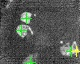
\includegraphics[keepaspectratio,height=4cm]{threshDistance10}
		\caption{Threshold Ergebnis des Distanztest mit 10cm Abstand}
		\label{fig:thresholdDistance10}
	\end{subfigure}\hfill
	\begin{subfigure}{\linewidth}
		\centering
		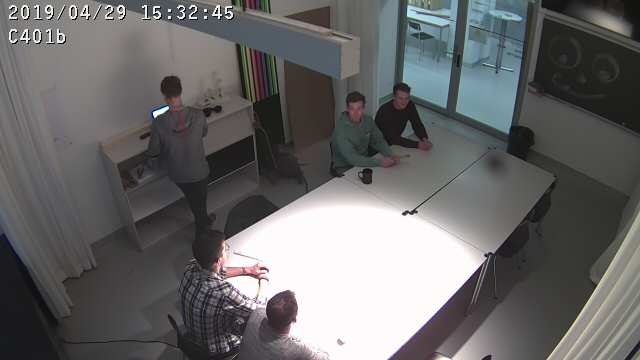
\includegraphics[keepaspectratio,height=3cm]{GroundDistance10}
		\caption{Ground-Truth Distanzexperiment mit 10cm Abstand}
		\label{fig:groundDistance10}
	\end{subfigure}
	\caption{Distanzexperiment 10cm}
	\label{fig:Distance10}
\end{figure}

\begin{figure}[H]
	\begin{subfigure}{.45\linewidth}
		\centering
		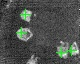
\includegraphics[keepaspectratio,height=4cm]{CNNDistance30}
		\caption{\gls{CNN} Ergebnis des Distanztest mit 30cm Abstand}
		\label{fig:cnnDistance30}
	\end{subfigure}\hfill%
	\begin{subfigure}{.45\linewidth}
		\centering
		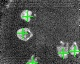
\includegraphics[keepaspectratio,height=4cm]{threshDistance30}
		\caption{Threshold Ergebnis des Distanztest mit 30cm Abstand}
		\label{fig:thresholdDistance30}
	\end{subfigure}\hfill%
	\begin{subfigure}{\linewidth}
		\centering
		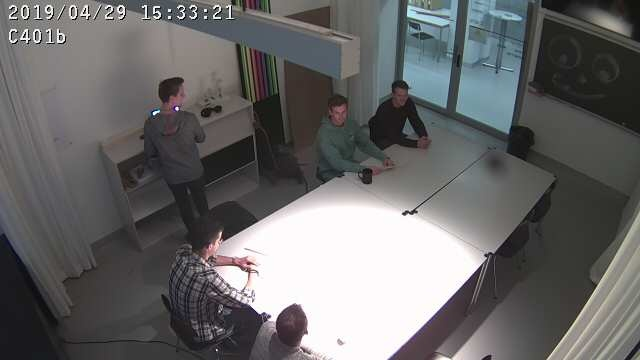
\includegraphics[keepaspectratio,height=3cm]{GroundDistance30}
		\caption{Ground-Truth}
		\label{fig:groundDistance30}
	\end{subfigure}
	\caption{Distanzexperiment 30cm}
	\label{fig:Distance30}
\end{figure}

\section{Grösse Des Objekts auf dem Bild}
\label{sec:objectSize}
Eine Spezialität des Sitzungszimmers, das zur Verfügung gestellt wurde, ist, dass die Höhe der Decke verändert werden kann. Da die Infrarotkameras an der Decke montiert sind, wurde dies als Möglichkeit genutzt um zu testen wie die Algorithmen auf grössen der Objekte im Bild reagieren. 

\subsection{Versuchsaufbau}

Die verstellbare Decke des Sitzungszimmers wurde auf die vom Mobiliar zugelassene Minimalhöhe, ca. 255cm, heruntergefahren. Danach wurden Infrarotbilder von Testpersonen an verschiedenen Positionen aufgenommen (siehe Abbildung \ref{fig:ground255cm}). Anschliessend wurde die Decke maximal hochgefahren, etwa 400cm, und noch einmal Bilder aufgezeichnet.

\begin{figure}[H]
	\centering
	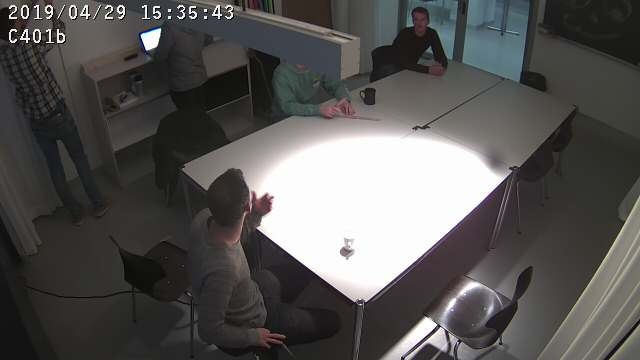
\includegraphics[height=4cm]{ground255cm}
	\caption{Sitzungszimmer mit Decke auf 255cm}
	\label{fig:ground255cm}
\end{figure}

\subsection{Resultate}

{
	\renewcommand{\arraystretch}{1.3}
	\begin{table}[H]
		\scriptsize
		\centering
		\begin{tabularx}{.6\textwidth}{Xrr}
			\hline
			\multicolumn{3}{c}{\textbf{CNN Ergebnisse des Objektgrössenexperiments}}\\
			\hline
			\textbf{Metriken} & \textbf{255cm} & \textbf{400cm}\\
			\hline
			\textbf{Gesamtanzahl Personen in Bilder} & 78 & 44 \\
			\hline
			\textbf{Korrekt identifizierter Personen} & 77 & 42\\
			\hline
			\textbf{Falsche Treffer} & 7 & 1\\
			\hline
			\textbf{Nicht erkannte Personen} & 1 & 2\\
			\hline
			\textbf{Recall} & 98.7\% & 95.5\%\\
			\hline  
			\textbf{Precision} & 91.7\% & 97.7\%\\
			\hline
			\textbf{F1-Score} & 95.1\% & 96.6\%\\
			\hline
		\end{tabularx}
		\caption{CNN, Ergebnisse des Distanztests}
		\label{tbl:objectSizeCNN}
	\end{table}
	\begin{table}[H]
		\scriptsize
		\centering
		\begin{tabularx}{.6\textwidth}{Xrr}
			\hline
			\multicolumn{3}{c}{\textbf{Threshold-Methode Ergebnisse des Objektgrössenexperiments}}\\
			\hline
			\textbf{Metriken} & \textbf{255cm} & \textbf{400cm}\\
			\hline
			\textbf{Gesamtanzahl Personen in Bilder} & 78 & 44 \\
			\hline
			\textbf{Korrekt identifizierter Personen} & 77 & 44\\
			\hline
			\textbf{Falsche Treffer} & 8 & 1\\
			\hline
			\textbf{Nicht erkannte Personen} & 1 & 0\\
			\hline
			\textbf{Recall} & 98.7\% & 100\%\\
			\hline  
			\textbf{Precision} & 90.6\% & 97.8\%\\
			\hline
			\textbf{F1-Score} & 94.5\% & 98.9\%\\
			\hline
		\end{tabularx}
		\caption{Threshold-Methode, Ergebnisse des Distanztests}
		\label{tbl:objectSizeThresh}
	\end{table}
}

\subsection{Evaluation}
Beide Algorithmen können die Personen in beiden Situationen noch immer in über 95\% der Fälle identifizieren. Werden die Objekte jedoch zu gross kann es bei beiden dazu führen, dass Personen doppelt gezählt werden. Da eine solch kleine Distanz aber nur schon durch das sehr kleine Sichtfeld für einen solchen Anwendungsfall nicht praktikabel ist, ist dies kein Problem, das weiter verfolgt werden müsste.\\
Werden die Objekte kleiner stellt dies für beide Algorithmen kein messbares Problem dar, solange die Charakteristiken noch klar erkennbar sind und die Personen eine Fläche von mindestens 10x10 Pixel einnehmen. Ein Test um die Grenze in diesem Bereich zu testen konnte in den zur Verfügung stehenden Räumlichkeiten leider nicht durchgeführt werden.\\
Möchte man jedoch die reale Position der Personen aus dem Bild berechnen, müsste die Deckenhöhe zusätzlich berechnet oder gemessen werden.

\begin{figure}[H]
	\begin{subfigure}{.45\linewidth}
		\centering
		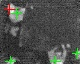
\includegraphics[keepaspectratio, height=4cm]{CNN255}
		\caption{Ergebnis des CNN mit Deckenhöhe 255cm}
		\label{fig:cnn255}
	\end{subfigure}\hfill%
	\begin{subfigure}{.45\linewidth}
		\centering
		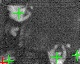
\includegraphics[keepaspectratio, height=4cm]{thresh255}
		\caption{Ergebnis der Threshold-Methode mit Deckenhöhe 255cm}
		\label{fig:thresh255}
	\end{subfigure}\hfill%
	\begin{subfigure}{.45\linewidth}
		\centering
		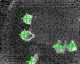
\includegraphics[keepaspectratio, height=4cm]{CNN400}
		\caption{Ergebnis des CNN mit Deckenhöhe 400cm}
		\label{fig:cnn400}
	\end{subfigure}\hfill%
	\begin{subfigure}{.45\linewidth}
		\centering
		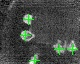
\includegraphics[keepaspectratio, height=4cm]{thresh400}
		\caption{Ergebnis der Threshold-Methode mit Deckenhöhe 400cm}
		\label{fig:thresh400}
	\end{subfigure}\hfill%
	\begin{subfigure}{.45\linewidth}
		\centering
		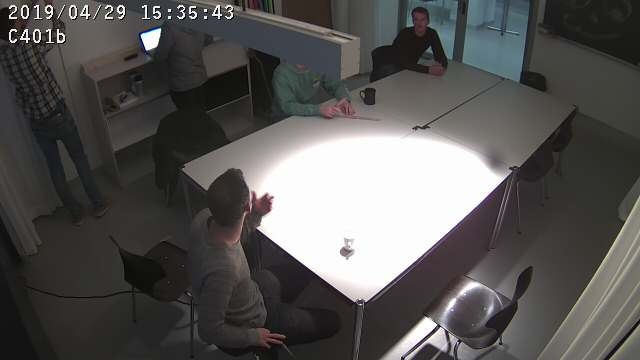
\includegraphics[keepaspectratio, height=4cm]{ground255cm}
		\caption{Ground Truth Deckenhöhe 255cm}
		\label{fig:ground255}
	\end{subfigure}\hfill%
	\begin{subfigure}{.45\linewidth}
		\centering
		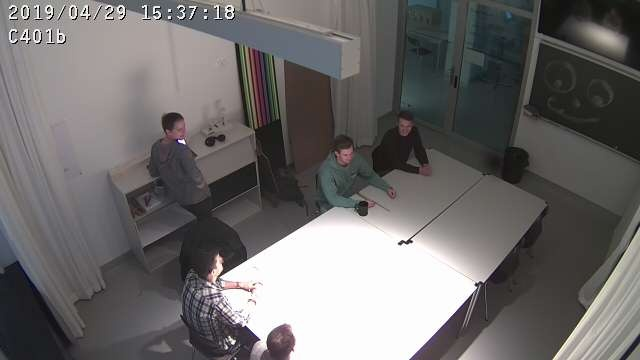
\includegraphics[keepaspectratio, height=4cm]{ground400cm}
		\caption{Ground Truth Deckenhöhe 400cm}
		\label{fig:ground400}
	\end{subfigure}
\end{figure}


\section{Kleider}
\label{sec:cloths}

Infrarotbilder zeigen die Wärmeabstrahlung der verschiedenen Objekte im Bild. Wird eine Wärmequelle isoliert, verschwindet sie auf dem Infrarotbild. Genau das passiert, wenn stark isolierende Kleider getragen werden. Da in dieser Arbeit die Vogelperspektive analysiert wird, haben vor allem Kopfbedeckungen, Schals und Jacken einen grossen Einfluss. 

\subsection{Versuchsaufbau}

Eine Testperson hielt sich an den in den Abbildungen \ref{fig:clothPositions} zu sehenden Positionen im Raum auf und trug verschiedene Kleidungsstücke. Dabei wurden eine Mütze, ein Schal und eine Jacke einzeln und alle kombiniert von der Testperson getragen.

\begin{figure}[H]
	\centering
	\begin{subfigure}{.45\linewidth}
		\centering
		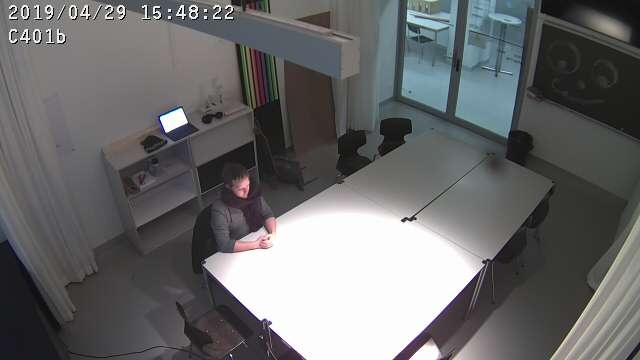
\includegraphics[keepaspectratio, height=3cm]{clothPos1}
		\caption{Position 1}
	\end{subfigure}
	\begin{subfigure}{.45\linewidth}
		\centering
		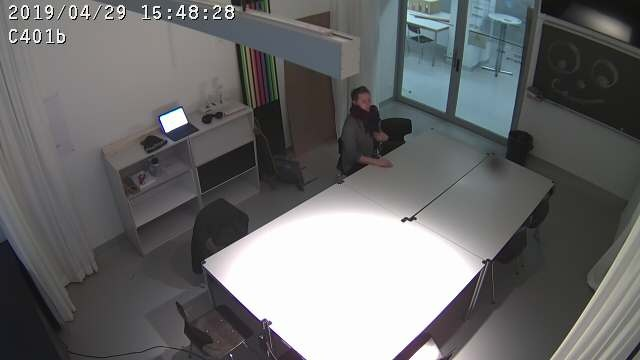
\includegraphics[keepaspectratio, height=3cm]{clothPos2}
		\caption{Position 2}
	\end{subfigure}
	\begin{subfigure}{.45\linewidth}
		\centering
		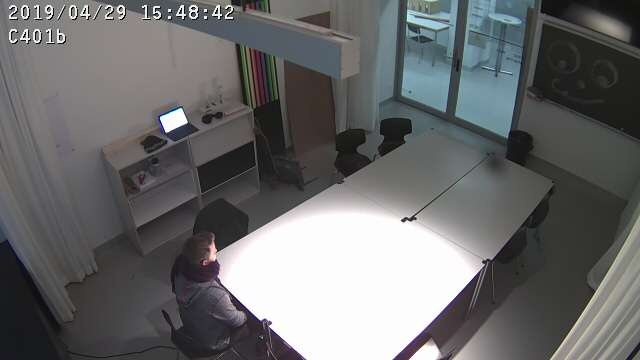
\includegraphics[keepaspectratio, height=3cm]{clothPos3}
		\caption{Position 3}
	\end{subfigure}
	\caption{Positionen der Testperson im Kleidungs Experiment}
	\label{fig:clothPositions}
\end{figure}

\subsection{Resultate}

{
	\renewcommand{\arraystretch}{1.3}
	\begin{table}[H]
		\centering
		\scriptsize
		\begin{tabularx}{.9\textwidth}{Xrrrr}
			\hline
			\multicolumn{5}{c}{\textbf{CNN Ergebnisse Kleider Experiment}}\\
			\hline
			\textbf{Metriken} & \textbf{Kappe} & \textbf{Jacke} & \textbf{Schaal} & \textbf{Alle drei Kleidungsstücke}\\
			\hline 
			\textbf{Gesamtanzahl Personen in Bilder} & 19 & 18 & 21 & 3\\
			\hline
			\textbf{Korrekt identifizierter Personen} & 23 & 0 & 15 & 0\\
			\hline
			\textbf{Falsche Treffer} & 0 & 0 & 0 & 0\\
			\hline
			\textbf{Nicht erkannte Personen} & 4 & 18 & 6 & 3\\
			\hline
			\textbf{Recall} & 82.6\% & -- & 71.4\% & -- \\
			\hline  
			\textbf{Precision} & 100\% & -- & 100\% & -- \\
			\hline
			\textbf{F1-Score} & 90.5\% & -- & 83.3\% & -- \\
			\hline
		\end{tabularx}
		\caption{Ergebnisse des CNN, des Kleider Experiments}
		\label{tbl:clothCNN}
	\end{table}
	\begin{table}[H]
		\centering
		\scriptsize
		\begin{tabularx}{.9\textwidth}{Xrrrr}
			\hline
			\multicolumn{5}{c}{\textbf{CNN Ergebnisse Kleider Experiment}}\\
			\hline
			\textbf{Metriken} & \textbf{Kappe} & \textbf{Jacke} & \textbf{Schaal} & \textbf{Alle drei Kleidungsstücke}\\
			\hline 
			\textbf{Gesamtanzahl Personen in Bilder} & 23 & 18 & 21 & 3\\
			\hline
			\textbf{Korrekt identifizierter Personen} & 23 & 5 & 16 & 0\\
			\hline
			\textbf{Falsche Treffer} & 12 & 0 & 1 & 3\\
			\hline
			\textbf{Nicht erkannte Personen} & 4 & 13 & 5 & 0\\
			\hline
			\textbf{Recall} & 100\% & 27.8\% & 76.2\% & -- \\
			\hline  
			\textbf{Precision} & 65.7\% & 100\% & 94.1\% & -- \\
			\hline
			\textbf{F1-Score} & 79.3\% & 43.5\% & 84.2\% & -- \\
			\hline
		\end{tabularx}
		\caption{Ergebnisse der Threshold-Methode, des Kleider Experiments}
		\label{tbl:clothThresh}
	\end{table}
}



\subsection{Evaluation}
Kleider beeinflussen die Performance der Algorithmen massiv. Trägt eine Person z.B. eine Mütze, wird sie vom \gls{CNN} noch zu 83\% erkannt. Bei der Threshold-Methode sind es zwar 100\%,führt aber dazu, dass eine Person zwei Treffer erzeugt (siehe Abbildung \ref{fig:thresholdClothHat}).\\
\\
Wenn ein Schal getragen wird, sinkt der Recall auf 71\% beim \gls{CNN} und 76\% bei der Threshold-methode. Betrachtet man Abbildung \ref{fig:scarfIR} sieht man deutlich, wie der Schal einen Teil der Wärme der Person verdeckt.\\
\\
Das Tragen einer Jacke macht es für die Algorithmen beinahe unmöglich die Personen zu erkennen. Die Person wird nur noch in wenigen Fällen erkannt. Da die Fläche der Abwärme einer Person so nur noch wenige Pixel beträgt, wird es schwierig diese von fremden Wärmequellen zu unterscheiden.\\

\begin{figure}[H]
	\centering
	\begin{subfigure}{.45\linewidth}
		\centering
		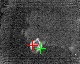
\includegraphics[keepaspectratio, height=4cm]{thresholdClothHat}
		\caption{Resultat der Threshold-Methode des Experiments mit Kopfbedeckung}
		\label{fig:thresholdClothHat}
	\end{subfigure}\hfill%
	\begin{subfigure}{.45\linewidth}
		\centering
		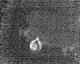
\includegraphics[keepaspectratio, height=4cm]{scarfIR}
		\caption{Infrarotbild einer Person die einen Schal trägt}
		\label{fig:scarfIR}
	\end{subfigure}\hfill%
	\caption{Infrarotbilder aus dem Kleider Experiment}
\end{figure}

\noindent
Die Tests mit allen Kleidungsstücken zeigen schon bei der manuellen, visuellen Analyse der Abbildung \ref{fig:rawClothAll}, dass wenn Jacke, Mütze und Schal zusammen getragen werden, dass die Person nicht mehr erkennbar ist.

\begin{figure}[H]
	\begin{subfigure}{.45\linewidth}
		\centering
		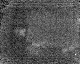
\includegraphics[keepaspectratio, height=4cm]{rawClothAll}
		\caption{Infrarotbild des Experiments mit Jacke, Mütze und Schal}
		\label{fig:rawClothAll}
	\end{subfigure}\hfill%
	\begin{subfigure}{.45\linewidth}
		\centering
		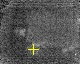
\includegraphics[keepaspectratio, height=4cm]{clothAll}
		\caption{Position der Person}
		\label{fig:AlgorithmsClothAll}
	\end{subfigure}\hfill%
	\begin{subfigure}{\linewidth}
		\centering
		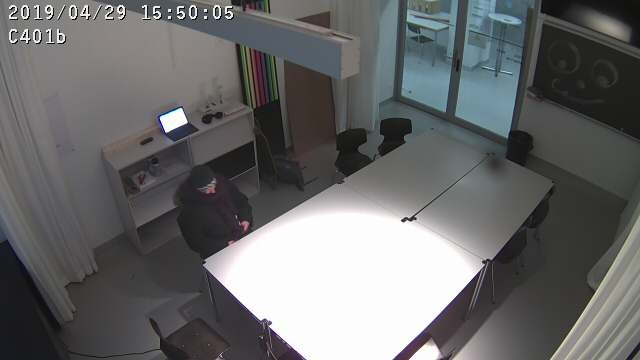
\includegraphics[keepaspectratio, width=.5\linewidth]{GroundClothAll}
		\caption{Ground-Truth des Experiments mit allen Kleidern}
		\label{fig:groundTruthClothAll}
	\end{subfigure}
	\caption{Experiment mit Jacke Mütze und Schal}
	\label{fig:AllCloth}
\end{figure}

